\newcommand{\name}{K223 -- Nuclear $\boldmath{\gamma}$-$\boldmath{\gamma}$ angular correlations }
\documentclass[11pt,a4paper,notitlepage]{scrartcl}
\usepackage{DasPaket}
\title{ Advanced Laboratory Course}
\subtitle{\name  \\ \hrulefill}
\date{April 08 2021 \\}
%\date{Date of Experiment \\ \sectionlinetwo{black}{88}}
\author[*]{\textsc{Dominic Schüchter}}
\author[$\dagger$]{\textsc{Jakob Krause}}
\affil[*]{\href{mailto:dschuechter@uni-bonn.de}{\faEnvelope  \hspace*{0.1cm}dschuechter@uni-bonn.de} {\color{black}$|$} \href{https://github.com/dschuechter}{\faGithub  \hspace*{0.1cm}dschuechter}}
\affil[$\dagger$]{\href{mailto:krause.jakob@uni-bonn.de}{\faEnvelope  \hspace*{0.1cm}krause.jakob@uni-bonn.de} {\color{black}$|$} \href{https://github.com/krausejm}{\faGithub  \hspace*{0.1cm}krausejm}}
\usepackage{blindtext}
\usepackage{amsmath}
\usepackage{braket}
\usepackage{booktabs}
\graphicspath{{figs/}}
\addbibresource{Literatur.bib}

\begin{document}

\maketitle
\vspace{-.8cm}
\thispagestyle{empty}
\begin{center}
\includegraphics[width=\linewidth]{titlepic}
\vspace{-.2cm}

\rule{12cm}{1pt} \\\vspace{-.6cm} \rule{10cm}{1pt}
\end{center}



\begin{abstract}
	In this report we investigate the angular correlation between two photons that are emitted in the process of a cascaded decay of $^{60}$Co. We use a FAST-SLOW coincidence circuit with scintillation detectors for this measurement. We compare our results to theoretical predictions.
\end{abstract}
\begin{center}
	 \rule{10cm}{1pt} \\\vspace{-.6cm} \rule{12cm}{1pt}
\end{center}

\setcounter{page}{-1}
\newpage

\tableofcontents
\thispagestyle{empty}
\newpage
\section{Introduction}
In this report we investigate angular correlations of $\gamma$ emission in the cascaded decay of $^{60}$Co. One can use this method to determine nuclear spins which has already been done for $^{60}$Co so we are left with confirming predictions. In section \ref{sec:theo} we qualitatively explain the theoretical background of angular $\gamma\gamma$ correlations. Next, in section \ref{sec:exp} we give the experimental setup to make correlation measurements (FAST-SLOW circuit) to proceed to section \ref{sec:anal}, where we display our measurements and analysis; first the FAST-SLOW coincidence circuit has to be calibrated, after this we can start with our measurements. Because of limited time we have to make compromises during our measurement regarding statistical precision and quantity of data and carefully make a choice what to prefer and why. We also measure for systematical errors. Lastly we draw a conclusion in section \ref{sec:conc}.

\section{Theory}
\label{sec:theo}
We will now briefly give the theory which is necessary to understand the aim of the experiment.
\subsection{Angular correlation of a $\gamma\gamma$ cascade}
Nuclei are bound systems and can be excited, analogous to atoms. Nuclei are often in a excited state after a decay which changed the compositions of the nucleus. To reach its ground state it has to decay via the emission of $\gamma$-radiation. If a multilevel decay is observed where the middle level(s) are very short lived ($\mathcal{O}(\si{\pico\s})$) it is a so called cascaded decay. Naively one could expect that the angular distribution of photons stemming from a cascaded decay be isotropic. This is not always the case; consider the cascaded decay of some (hypothetical) nucleus via the spin levels $0-1-0$. Then the possible spin states are (notation $\ket{I,m_I}$)
$$\ket{0,0}\underset{\gamma_1}{\to}
\begin{Bmatrix}
	\ket{1,+1}\\
	\ket{1,0}\\
	\ket{1,-1}\\
\end{Bmatrix}
\underset{\gamma_2}{\to}\ket{0,0}.$$
Since momentum has to be conserved the emitted photons carry the difference in momentum away. If we now detect $\gamma_1$ we fix the $z$ axis to be in the direction of $\gamma_1$ which demands $\Delta m_1=\pm1$ since the photon can only have $m_{\gamma_1}=\pm1$. This in turn however leads to an underpopulation of the intermediate state $\ket{1,0}$. A coincident measurement of both photons will now lead to an anisotropic angular distribution of the coincidence rate because the distribution of $m_{\gamma_2}$ is anisotropic. Quantitatively this is expressed by the correlation rate  in dependence of the polar angle $W(\theta)$ which can be obtained by looking at transition probabilities employing \textsc{Clebsch-Gordan} coefficients and emission characteristics of photons to be \cite{nuclear} \begin{equation}
	W(\theta)\propto1+\cos^2\theta.
\end{equation} This subsection was oriented at \cite{nuclear}.
\subsection{Cascaded decay of $^{60}$Co}
By studying angular correlations one can determine the spin of the energy levels involved. This way the spins of the $^{60}$Co decay products were determined \cite{siegbahn} to be $4-2-0$, see figure \ref{fig:Decay}.
\begin{figure}[htbp]
	\centering
	\includegraphics[width=.49\linewidth]{figs/decay}
	\includegraphics[width=.49\linewidth]{figs/decay_scheme}
	\caption{Decay schemes of $^{60}$Co, we see $E_{\gamma_1}=\SI{1.17}{\mega\eV}$, $E_{\gamma_2}=\SI{1.33}{\mega\eV}$. On the right the probabilities $P(m_I)$ of occupying the respective intermediate state $m_I$ are indicated \cite{nuclear}.}\label{fig:Decay}
\end{figure}
The $^{60}$Co decays ($\beta^-$-decay) with a life time of $t_{1/2}=5.26$ y which means it can continuously produce excited $^{60}$Ni$^*$. This in turn decays very quickly ($t_{1/2}=\mathcal{O}(\si{\pico\s})$) to its ground state under the emission of two photons. Because of the qualitatively discussed reasons in the previous subsection, a coincident measurement of these two photons will be anisotropic in the form \cite{nuclear}\begin{equation}
	W(\theta)=\text{const.}\left(1+A_2\cos^2\theta+A_4\cos^4\theta\right)=\text{const.}\left(1+\frac{1}{8}\cos^2\theta+\frac{1}{4}\cos^4\theta\right).
	\label{eq:wtheta}
\end{equation}
Equation \ref{eq:wtheta} only holds for ideal detectors. In reality the coefficients have to be corrected because of the finite solid angle range d$\alpha$ they cover in addition to only the angle range in $\theta$ by \cite{siegbahn} \begin{align}
	A_k=A_k^{\text{exp}}/Q_k^2=A_k^{\text{exp}}\cdot\frac{J_0}{J_k}, && J_k=\int_0^{1}\text{d}\cos\alpha\left\{\epsilon(E,\alpha)P_k(\cos\alpha)\right\}.
\end{align} Here $\epsilon$ is the efficiency and $P_k$ are the \textsc{Legendre} polynomials. The $Q_k$ coefficients have been calculated in dependence of the distance of emitter to detector and the energy of the photons and are tabulated in \cite{siegbahn} which we will use later on.
\section{Experimental Setup}
\label{sec:exp}
In this section we will give a brief introduction in the experimental setup and explain the electronic parts and techniques we used. It follows the structure of the handbook \cite{manual}.

Figure \ref{fig:aufbau} shows a schematic of the setup. If a $\gamma$-$\gamma$-cascade takes place, the time difference of the photon creation is far smaller than our time resolution. Therefore we can assume, that both photons arrive simultaneously (coincident) in the detectors. Two detectors, one fixated and the other movable, are placed on a circular table at the same distance to the source. Both detectors are NaI(Tl) Scintillation Detectors (ORTEC 905 Series). The chosen distance is each 5cm to the source. The distance choice is a rather important one, because the source as well as the detector are extensive objects and not punctual. With increasing distance grows the resolution, because the detector covers smaller angles, while the counting rate decreases by $1/r^2$ and a coincidence rate by $1/r^4$. One could choose a rather big distance and make longer measurements, but this was not an option because of time reasons. The scintillators have each two outputs, namely the \texttt{SLOW}- and the \texttt{FAST}-output. The fast output delivers a sharp but small signal that wasn't amplified as much by the photomultiplier, which is ideal for time measurements. The slow signal was strongly amplified in comparison and is ideal for energy measurements. Both signal from each detector are inserted in two separated circuits:
\begin{itemize}
	\item \textbf{SLOW-Circuits} (energy selection):  The slow circuit consists of an amplifier \texttt{A} and a Single Channel Analyzer \texttt{SCA}. The amplifier converts the incoming signal into a box shaped signal with the voltage amplitude height proportional to the energy. The \texttt{SCA} then filters a set voltage window.
	\item \textbf{FAST-Circuit} (time selection): The fast circuit consists of an constant fraction discriminator \texttt{CFD} and a delay \texttt{D}. The constant fraction discriminator triggers by design for different signals with different rising times at the same moment. This is a big advantage against for example threshold triggering and therefore good for time measurements. The \texttt{CFD} has an additional threshold discriminator that will be set in a way, that coincidences aren't effected while noise is suppressed. The fast circuit comes together in a fast coincidence element \texttt{FC}. With the variable delay \texttt{D3}  one can tune the coincidence time.
\end{itemize}
Both Circuits are combined in a universal coincidence element \texttt{UC}. Since the fast circuit is as the name suggest faster then the slow one, one finds behind the fast coincidence a gate and delay generator \texttt{D$^2$-G$^2$}. To further tune the coincidence there are two delays at every slow arm before the \texttt{UC}. If one slow arm triggers a decay at the set energy window, the associated counter (\texttt{count.1/2}) increases. If both slow signals are coincident with the fast coincidence then the counter \texttt{count.3} increases. So one measures the three counting rates over an integration time $t$ that is set at the timer \texttt{T}. This system is not free of random coincidences. Therefore an additional measurement has to be done.

\begin{figure}[htpb]
	\centering
	\includegraphics[width=0.7\linewidth]{./figs/Setup.png}
	\caption{Principle schematic of the experiment \cite{manual}}\label{fig:aufbau}
\end{figure}

\section{Measurements and Analysis}
\label{sec:anal}
In this section we will describe how we setup the experiment and took the measurements. Furthermore we will do the data analysis and derive experimental results.

\subsection{Preparation of the setup}
We will begin with the preparation of the setup. Since at this point the position of the detectors is not important, we just let it as it was at about 90$^\circ$. This gets important at the main measurement.
\subsubsection{Energy Branch - Adjusting the Gain}
Because larger signals yield to smaller disturbances \cite{manual} we amplify the slow signals by the amplifiers \texttt{A1} and \texttt{A2}. The output of the amplifiers is linear up to 9V \cite{manual}. Figure \ref{fig:amp_osci} shows two screen shots of the amplified outputs. As one can see, the two main transitions as described in the decay scheme \ref{fig:Decay} have the highest contrast on the oscilloscope screen. We amplified those signals until they reached approximate the 8V signal height.
\begin{figure}[htbp]
	\begin{subfigure}{0.49\linewidth}
		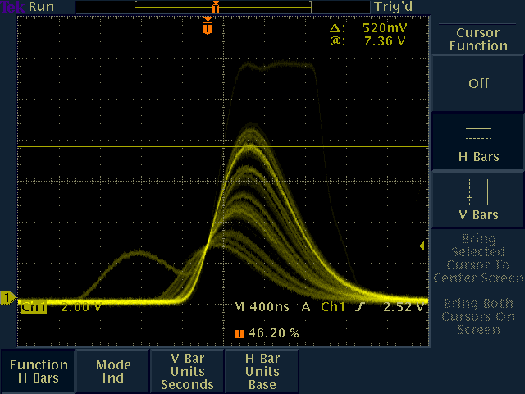
\includegraphics[width=\linewidth]{figs/osci_pics/Amp1.pdf}
		\caption{Amplifier \texttt{A1} -- signal output}
	\end{subfigure}
		\begin{subfigure}{0.49\linewidth}
		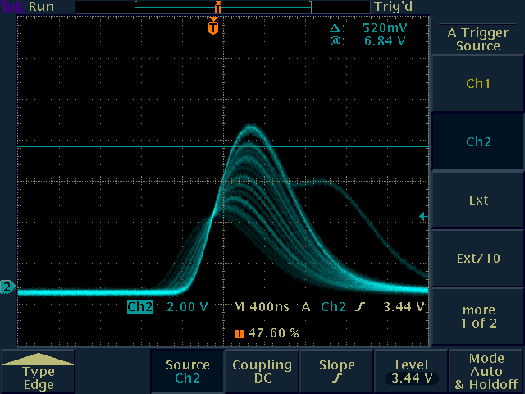
\includegraphics[width=\linewidth]{figs/osci_pics/Amp2.pdf}
		\caption{Amplifier \texttt{A2} signal output}
	\end{subfigure}
	\caption{Amplified signals in the slow circuit}\label{fig:amp_osci}
\end{figure}

\subsubsection{Calibrating the Single Channel Analyzer, selecting the gamma events}
To calibrate the single channel analyzer, we set the \textsc{SCA's} to \texttt{window}-mode. In this mode one can set a window and variate the lower limit. Therefore we can scan the energy spectrum evenly. One could also set upper and lower limits, but therefore the error would increase. Also to have comparable results in the form of a histogram one of course hast to choose equal bin widths. We chose a window width of $20$ ticks allowing for a detailed scan of the spectrum and also enough statistics within each bin. A plot during the lab session confirmed our choice was reasonable since we could observe all characteristic points of a $\gamma$ spectrum in a scintillator. The peaks of the transitions $\gamma_1$,$\gamma_2$ were clearly visible which is the most important aspect since we need to specify the SCA window. We created a (nice looking) histogram for this report for each step and plotted it in figure \ref{fig:SCA_window}. The total integration time for each bin was 4s. The two highest peaks, after the compton edge (at about 500 ticks) are the signals of the $\gamma$-$\gamma$-cascade. This can be said, because we see a typical gamma spectrum with \textsc{Compton} scattering (0-500 ticks), \textsc{Compton} edge (500 ticks) and escape peak (180 ticks). On top comes the fact, that the energies of our cascade are 1.17 MeV and 1.33 MeV. Their energy difference is about 160 MeV. In the spectrum both peaks are about 100 ticks apart. With this in mind one tick would translate to 1.6 MeV. Therefore  the 1173.237 MeV peak should be at $\frac{1.17\text{MeV}}{1.6\text{MeV/tick}}\approx 733$ ticks and the 1332.501 MeV peak at $\frac{1.33\text{MeV}}{1.6\text{MeV/tick}}\approx 833$ ticks. If we assume that the 0 point translates to 0 MeV then is this coarse estimate a fairly good result. We then isolated the peaks with a little scope of the lower limit and set the upper limit to the maximum. One could have done an energy calibration, but since this is only about filtering the signals and done really coarsely, we can go on to the fast branch. We set the SCA window to channels 600-1000.
\begin{figure}[htbp]
	\centering
	\includegraphics[width=.49\linewidth]{figs/SCA/SCA1.pdf}
	\includegraphics[width=.49\linewidth]{figs/SCA/SCA2.pdf}
	\caption{SCA window selection. Errors are neglected, since this calibration is only qualitative.}\label{fig:SCA_window}
\end{figure}

\subsubsection{Timing Branch - Adjustment of the Constant-Fraction-Discriminator (\texttt{CFD})}
To filter noise without influencing the actual signal, we vary the threshold-discriminator of the \texttt{CFD}'s and measure directly the counting rates $N$ with and without a source. The integration time was set to 4s. We then plotted the counting rates against the threshold-discriminating settings which can be seen in figure \ref{fig:CFD_adjust}.

\begin{figure}[H]
	\centering
	\begin{subfigure}{0.3\linewidth}
		\includegraphics[width=\linewidth]{figs/CFD/CFD1.pdf}
	\end{subfigure}
		\begin{subfigure}{0.3\linewidth}
		\includegraphics[width=\linewidth]{figs/CFD/CFD2.pdf}
	\end{subfigure}
	\caption{\texttt{CFD} configuration}\label{fig:CFD_adjust}
\end{figure}

One can see a big change between the values of 0 (no threshold-discrimination) and the \texttt{CFD} setting 10. After this jump there is a almost flat area where the counting rate without a source decreases strong and the counting rate with source stays almost constant on the logarithmic scale. Therefore we set the value of the threshold-discriminator to 20. Since this value is set on a potentiometer and we don't have further documentation, this numbers are non physical and only serve the purpose of calibration.

\subsubsection{Setting up the Fast Coincidence}\label{sec:fast_coincidences}
To setup the fast coincidence we have a constant delay \texttt{D} of 50 ns (wire delay) and a variable one \texttt{D3} available.

Before we quantify the delay \texttt{D3}, we visualized the out coming signals of both fast circuits on an oscilloscope and triggered on channel 2 (\texttt{CFD 2}) for an applied and misapplied variable delay \texttt{D3}. The screenshots are depicted in figure \ref{fig:CFD_trigger}.

\begin{figure}[H]
	\centering
	\begin{subfigure}{0.49\linewidth}
		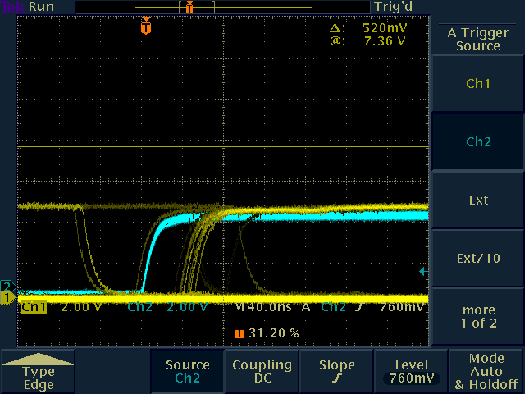
\includegraphics[width=\linewidth]{figs/osci_pics/TEK00002.pdf}
		\caption{variable delay set to 64ns}
	\end{subfigure}
	\begin{subfigure}{0.49\linewidth}
		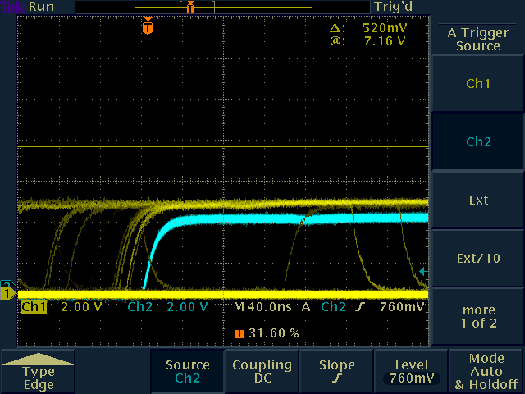
\includegraphics[width=\linewidth]{figs/osci_pics/TEK00003.pdf}
		\caption{variable delay set to 0ns}
	\end{subfigure}
	\caption{Oscilloscope screenshots with and without enabled variable delay.}\label{fig:CFD_trigger}
\end{figure}

If the delay is set to zero, no real coincidences (high contrast lines) can ever take place.

We then measured the counting rate behind the  fast coincidence -- after wiring everything back together --   for different delay settings of \texttt{D3} and with a applied resolving time of approximately 25 ns (we had to rely on experience from our tutor to set the potentiometer accordingly). In figure \ref{fig:prompt} is the resulting prompt curve depicted.


The first data points behave very unexpected, we find no explanation for this. Nevertheless we fit the expected function \eqref{eq:func} to the data and explicitly do not ignore "faulty" data points.  The fitted function does thus not very well describe the outer parts of our data.  We still consider the fit to be reasonably good since we are mostly interested in the very well fitting center of the data to estimate our resolving time. Since the goal was to find the sweet spot to measure the most possible coincidences, we set the delay to the center of the distribution at 42 ns allowing a broad margin to higher and lower delays for slightly delayed signals in the repective FAST branches.

The fitted function of the prompt curve
\begin{equation}\label{eq:func}
	f(t)=\frac{A_1}{2}\cdot\left(1+\text{erf}\left(\frac{t-t_0}{\sigma}\right)\cdot \text{erf}\left(\frac{t_1-t}{\sigma}\right)\right)+A_0
\end{equation}
has the parameters
\begin{itemize}
	\item $A_1=(1581.2\pm88.4)$ s$^{-1}$: Amplitude in proportion to the count rate of real coincidences
	\item $t_0=(27.5\pm0.8)$ ns and $t_1=(55.5\pm0.6)$ns: Box edges. Therefore is $\Delta t=t_1-t_0=(28.0\pm0.8)$ ns the true resolving time, agreeing with our first estimate
	\item $\sigma= (5.9\pm 0.4)$ ns: time resolution (detector specific property)
	\item $A_0=(216.8\pm20.0) $s$^{-1}$: Offset in proportion to the count rate of random coincidences
\end{itemize}

\begin{figure}[H]
	\centering
	\includegraphics[width=\linewidth]{figs/prompt/prompt.pdf}
	\caption{Prompt-Curve}\label{fig:prompt}
\end{figure}
With this, one can give an estimate for the quality of the measurement by calculating the fraction
$$\frac{A_0}{A_0+A_1}\approx 12\%$$
and derives by this percentage an idea of the influence of the random coincidence. The amount of background (random coincidences) is therefore small enough to let the resolving time as is. If we would have chosen a larger or smaller resolving time, the curve would have a wider or narrower plateau containing significantly more random coincidences or less random but also less true coincidences. In either case this will raise the relative frequency of random coincidences.

\subsubsection{Setting up the Slow Coincidence}
The universal coincidence only works, as the name suggests, if the coincidence of all signals is given. Therefore we use the \texttt{D$^2$-G$^2$} to delay the signal from the \texttt{FC} and displace the individual slow branch signals with their associated delays \texttt{D1/2} in a way, that the signals are coincident and the leading edges match up. In principle we only need maximal alignment of the two signals. But to be able to set a coincident point for all three signals of which only two could be displayed simultaneously on the oscilloscope we chose the leading edge as an easy reference point. For this we visualized the signals again on an oscilloscope as depicted in figure \ref{fig:universal_coincidence}. With everything setup, we can now connect all three outputs to the universal coincidence \texttt{UC} and start measuring.
\begin{figure}[H]
	\centering
	\begin{subfigure}{0.49\linewidth}
		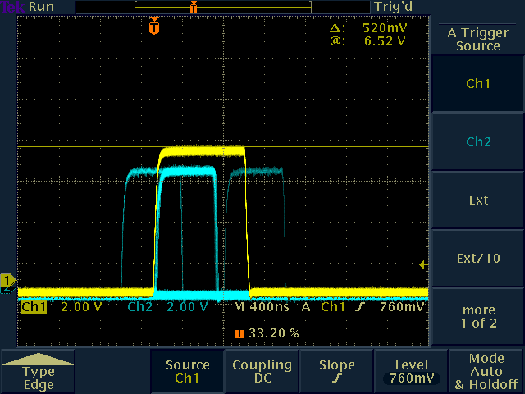
\includegraphics[width=\linewidth]{figs/osci_pics/UC1.pdf}
		\caption{\texttt{SCA}1}
	\end{subfigure}
	\begin{subfigure}{0.49\linewidth}
		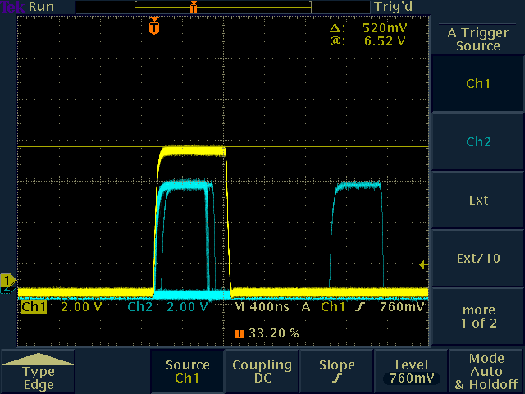
\includegraphics[width=\linewidth]{figs/osci_pics/UC2.pdf}
		\caption{\texttt{SCA}2}
	\end{subfigure}
	\caption{Coincidence of the \texttt{SCA}-signals (Channel 2 -- blue) with the \texttt{FC} signal (Channel 1 -- yellow)}\label{fig:universal_coincidence}
\end{figure}
\subsection{Main Measurement}
Our goal was to measure the angular correlation of the $\gamma$-$\gamma$-cascade. Since we had limited measuring time and the detectors/electrons tend to get influenced over time, we created the following plan. 

We wanted to cover the following angles 
\begin{equation*}
	\theta\in\{\color{red}90^\circ\color{black},105^\circ,120^\circ,\color{red}135^\circ\color{black},150^\circ,165^\circ,\color{red}180^\circ\color{black},195^\circ,210^\circ,\color{red}225^\circ\color{black},240^\circ,255^\circ,\color{red}270^\circ\color{black}\}
\end{equation*}
The red marked angles are most important, because they define the critical points of the curve. Therefore we measured them 5 times. The other angles (black) were measured twice each.
The measurement was done in the following order with an integration time of 200s for each angle:
\begin{enumerate}
	\item important angles (red)
	\item less important angles (black)
	\item important angles (red)
	\item important angles (red)
	\item important angles (red)
	\item less important angles (black)
	\item important angles (red)
\end{enumerate}

\subsubsection{Further adjustments}
We distributed our measurements this way to include the time dependence of the counting rates by taking the mean value and applying \textsc{Gaussian} error evolution. Figure \ref{fig:time_dependence} shows the time dependence for our two detectors. One can make the qualitative statement, that the detection rate is falling for \texttt{Det.1} over time, while the detection rates for the variable angles of \texttt{Det.2} are fluctuating. There is no trivial explanation for this behavior. One can only assume influences of the operating temperatures of the electronics.

\begin{figure}[htbp]
	\centering
	\begin{subfigure}{0.49\linewidth}
		\includegraphics[width=\linewidth]{figs/main/time_dependence_n1.pdf}
		\caption{\texttt{count.1} -- static detector}\label{fig:time_dependence_1}
	\end{subfigure}
	\begin{subfigure}{0.49\linewidth}
		\includegraphics[width=\linewidth]{figs/main/time_dependence_n2.pdf}
		\caption{\texttt{count.2} -- movable detector}\label{fig:time_dependence_2}
	\end{subfigure}
	\caption{The single detection count rates over time for the static detector \ref{fig:time_dependence_1} and the variable one \ref{fig:time_dependence_2}. We plotted all important angles. One can see that the count rates drop over time for the \texttt{Det.1}, while they are fluctuating for \texttt{Det.2}.}\label{fig:time_dependence}
\end{figure}

As said we measured every important angle 1000s in total and every other one 400s. Before just taking the mean value and proceeding to the analysis, we have to remove two more influences to the data.

First we have to filter out random coincidences. As explained in \ref{sec:fast_coincidences} and depicted in figure \ref{fig:CFD_trigger} one has to set the variable delay \texttt{D3} to 0 ns, so that no real coincidences can happen, see figure \ref{fig:prompt}. We leave the delays in the SLOW circuit \texttt{D1/D2} as they are. With this we collect an error since the SLOW circuit is designed to be coincident in the universal coincidence \texttt{UC} and may trigger it if the true coincidence arrives within the resolving time of a somehow still obtained true coincidence in the FAST circuit. Since we can safely assume no true coincidences in the FAST circuit will occur with our chosen delay we can neglect this error. We then measured the  number of random coincidences $N_r$ with an integration time of 1000 s and found:
$$N_r=2750 \Rightarrow n_r=\frac{N_r}{T}=\frac{2750}{1000\text{s}}=(2.75\pm0.05)\text{ s}^{-1}$$
where $n_r$ is the rate of random coincidences.

One can also calculate an estimation for the rate of random coincidences, by taking a look at the number of counts of both detectors
$$N_1=75451\cdot 10^2 \phantom{ nun } N_2=72191\cdot 10^2.$$
By building the count rate and multiplying it with the resolving time $\sigma=(28.0\pm0.8)$ ns one finds \cite{siegbahn}
$$n_r^{\text{estimate}}=2\sigma\cdot (N_1/T) \cdot (N_2/T)=(3.05\pm0.06)\text{ s}^{-1},$$
actually agreeing with our measured value within $3\sigma$ so we can conclude that our measurement of random coincidences was reasonable.
Taking this into account follows the counting rate of coincidences $n_C$ as:
$$n_C\rightarrow n_C-n_r$$

 If the source is not always at the same distance to the movable detector \texttt{Det.2}, a direct influence to the counting rate ($\propto1/r^2$) occurs. Therefore we have to apply here the second correction. We plotted the number of counts for each detector in dependence of the angle $\theta$. Since those counting rates include not coincident events, they should be evenly distributed. Figure \ref{fig:count2_angle} shows the angular dependence of the number of counts for detector \texttt{Det.2}.

To adjust the dataset, we have to choose a normalization point. We chose $N_2(\theta=180^\circ)$ -- every other datapoint would be as good as this one -- and applied it to the counting rate $n_C$
$$n_C\rightarrow (n_C-n_r)\cdot\frac{n_2(180^\circ)}{n_2(\theta)}$$
\begin{figure}
	\centering
	\includegraphics[width=\linewidth]{figs/main/count2.pdf}
	\caption{Counts of events for movable \texttt{Det.2} in dependence of the angle $\theta$}\label{fig:count2_angle}
\end{figure}

Now we are finally all set up and ready to analyze the data.

\subsubsection{Analysis}
With all corrections applied we then plotted the angle $\theta$ against the coincidence counting rate $n_C$ and fitted the function 
\begin{equation*}
	W(\theta)=a\left(1+A_2\cos^2\theta+A_4\cos^4\theta\right).
\end{equation*}
as depicted in figure \ref{fig:measurement}.

We obtained the fit parameters:
\begin{align*}
	a&=(40.406 \pm 0.110)\text{s}^{-1}\\
	A_2&=(0.108 \pm 0.015)\\
	A_4&=(0.022 \pm0.015)
\end{align*}

Since neither the source nor the detectors are punctual, we have to apply correction factors -- namely $Q_2$ and $Q_4$-- to our parameters.

Our experiment had the following properties:
\begin{itemize}
	\item Detector diameter: 2 inches
	\item Detector distance: 5cm
	\item Energy range: $\approx$ \SIrange{1}{1.5}{\mega\eV}
\end{itemize}
The correction factors were taken from Siegbahn \cite{siegbahn}. We chose the values for energies at $E=\{1,1.5\}$ MeV, since our $\gamma$-peaks lie in this value area. Our choice is listed in table \ref{tab:correction_factors}. The average and the standard deviation build our correction factors:
\begin{align*}
	Q_2=(0.90515\pm0.0005) && Q_4=(0.7100\pm0.0014)
\end{align*}

\begin{table}
	\centering
	\begin{tabular}{|c|c|c|}
		\hline
		$E$ / MeV& $Q_2$ & $Q_4$ \\
		\hline
		1.0& 0.9046 & 0.7086 \\
		1.5& 0.9057 & 0.7114\\
		avrg. &0.90515& 0.7100\\
		\hline
	\end{tabular}
	\caption{Correction factors by Siegbahn \cite{siegbahn}}\label{tab:correction_factors}
\end{table}
When we apply those correction factors, we find:
\begin{align*}
	A_2^{\text{corr.}}=\frac{A_2}{Q_2}=(0.138\pm0.019) && A_4^{\text{corr.}}=\frac{A_4}{Q_2}=(0.044\pm0.030)
\end{align*}
One expects values of $A_2=1/8=0.125$ and $A_4=1/24\approx 0.042$. The expected values lie in the errorbars of our measurement. Table \ref{tab:coeff} lists other possible spin states that could may be of interest as cited from \textsc{D.R. Hamilton} \cite{hamilton} in \cite{bdpaper}. Here only final states with $I=0$ are considered since $^{60}_{28}$ Ni is an even-even nucleus. We can safely exclude all other possibilities than the actually true one listed here within a margin of $>10\sigma$.

\begin{table}[H]
	\centering
\begin{tabular}{ccccc}
	\toprule
	$I_{2} (2)$ & $I_{3} (4)$ & Multipoles & $A_{2}$ & $A_{4}$ \\
	\hline 1 & 0 & Dipole-Dipole & 1 & 0 \\
	1 & 1 & Dipole-Dipole & $-1 / 3$ & 0 \\
	1 & 2 & Dipole-Dipole & $-1 / 3$ & 0 \\
	1 & 1 & Quadrupole-Dipole & $-1 / 3$ & 0 \\
	1 & 2 & Quadrupole-Dipole & $3 / 7$ & 0 \\
	1 & 3 & Quadrupole-Dipole & $-3 / 29$ & 0 \\
	2 & 3 & Dipole-Quadrupole & $-3 / 29$ & 0 \\
	2 & 2 & Dipole-Quadrupole & $3 / 7$ & 0 \\
	2 & 1 & Dipole-Quadrupole & $-1 / 3$ & 0 \\
	2 & 0 & Quadrupole-Quadrupole & $-3$ & 4 \\
	2 & 1 & Quadrupole-Quadrupole & 5 & $-16 / 3$ \\
	2 & 2 & Quadrupole-Quadrupole & $-15 / 13$ & $16 / 13$ \\
	2 & 3 & Quadrupole-Quadrupole & 0 & $-1 / 3$ \\
	2 & 4 & Quadrupole-Quadrupole & $1 / 8$ & $1 / 24$\\
	\bottomrule
\end{tabular}
\caption{Coefficients $A_2$,$A_4$ for other possible spin configurations, taken from \cite{bdpaper}. The multipoles indicate $\Delta m_I$ in the respective transitions, the numbers in brackets (x) represent the true values of the level}\label{tab:coeff}
\end{table}
\begin{figure}[htpb]
	\centering
	\includegraphics[width=0.9\linewidth]{figs/main/measurement.pdf}
	\caption{Corrected coincident count rate $n_C$ in dependence of the angle $\theta$}\label{fig:measurement}
\end{figure}

\newpage

\section{Conclusion}
In this experiment the decay cascade of $^{60}$Co was investigated. The emission angles of photons in a decay cascade are in general not uncorrelated. Considering the transition probabilities of the spin-levels taking part in the decay of $^{60}$Co one expects the coincidence rate $W(\theta)$ to follow the distribution $$W(\theta)\propto 1+\frac{1}{8}\cos^2\theta+\frac{1}{24}\cos^4\theta.$$   We made a coincidence measurement to determine the correlation between the two photons of the cascaded decay. We calibrated a FAST-SLOW coincidence circuit to make reliable measurements for selected angles. After correcting for random coincidences and misalignment of the setup we could determine \begin{align*}
	W(\theta)\propto 1+A_2\cos^2\theta+A_4\cos^4\theta &&\text{ with } A_2=0.139\pm0.019,&&A_4=0.044\pm0.030,
\end{align*}
agreeing within $1\sigma$ with the expectations. A major challenge during the execution of the experiment was the choice of measurement angles and according measurement time. Here we had to ponder between statistical precision and quantity of data points in total. Given the result we can assume our choice was reasonable. 
\label{sec:conc}

\appendix
\newpage
\section{Appendix}

\subsection{Remark on measurement errors}
We measured counts throughout the whole experiment. Every count $N$ is associated with an error $\sigma_N=\sqrt{N}$ (\textsc{Poisson} statistics). All errors are propagated using \textsc{Gaussian} error propagation.

\subsection{Measured data}
All data we measured was visualized in this report only in the form of plots. If there is need to view the data in detail it can be found in our \href{https://github.com/krausejm/advanced_lab_course}{GitHub repository}. 

\newpage
\printbibliography[heading=bibintoc]
\end{document}
